\documentclass[11pt]{article}

% ---------------------------------------------------------------------
% Packages
% ---------------------------------------------------------------------
\usepackage[margin=1in]{geometry}
\usepackage{amsmath,amssymb,amsthm}
\usepackage{mathtools}
\usepackage{graphicx}
\usepackage{booktabs}
\usepackage{multirow}
\usepackage{array}
\usepackage{xcolor}
\usepackage{hyperref}
\usepackage[capitalise]{cleveref}
\usepackage{algorithm}
\usepackage{algpseudocode}
\usepackage{tikz}
\usetikzlibrary{shapes.geometric, arrows.meta, positioning, fit, backgrounds, calc}
\usepackage{authblk}
\usepackage{caption}
\usepackage{subcaption}
\usepackage{enumitem}
\usepackage{natbib}
\bibliographystyle{plainnat}

\hypersetup{
    colorlinks=true,
    linkcolor=blue!60!black,
    citecolor=blue!60!black,
    urlcolor=blue!50!black
}

% ---------------------------------------------------------------------
% Theorem environments
% ---------------------------------------------------------------------
\newtheorem{theorem}{Theorem}[section]
\newtheorem{lemma}[theorem]{Lemma}
\newtheorem{corollary}[theorem]{Corollary}
\newtheorem{proposition}[theorem]{Proposition}
\newtheorem{definition}[theorem]{Definition}
\newtheorem{assumption}[theorem]{Assumption}
\newtheorem{conjecture}[theorem]{Conjecture}
\newtheorem{remark}[theorem]{Remark}

% ---------------------------------------------------------------------
% Custom macros
% ---------------------------------------------------------------------
\newcommand{\Aspec}{A_{\mathrm{spec}}}
\newcommand{\Atop}{A_{\mathrm{top}}}
\newcommand{\Asym}{A_{\mathrm{sym}}}
\newcommand{\Ahw}{A_{\mathrm{hw}}}
\newcommand{\Afull}{A(T,C,H)}
\newcommand{\R}{\mathbb{R}}
\newcommand{\C}{\mathbb{C}}
\newcommand{\N}{\mathbb{N}}
\newcommand{\E}{\mathbb{E}}
\newcommand{\norm}[1]{\left\lVert #1 \right\rVert}
\newcommand{\inner}[2]{\left\langle #1, #2 \right\rangle}
\newcommand{\fT}{f_T}
\newcommand{\fC}{f_C}
\newcommand{\Omc}{\Omega_C}
\newcommand{\Omt}{\Omega_T}

\title{\textbf{Q-ALIGN: A Task--Circuit Spectral--Topological Alignment Framework for Predicting and Designing Quantum Machine-Learning Architectures}}

\author[1]{Author One}
\author[1]{Author Two}
\author[2]{Author Three}
\affil[1]{Department of Computer Science, [Institution], [City, Country]}
\affil[2]{Department of Physics, [Institution], [City, Country]}

\date{}

\begin{document}

\maketitle

\begin{abstract}
Quantum machine learning (QML) architecture selection is still dominated by proxies borrowed from classical deep learning --- qubit count $n_q$, parameter count $P$, circuit depth $L$, and gate count $G$ --- none of which capture \emph{why} a given circuit ansatz suits a given task. We argue that suitability is governed by the \emph{alignment} between a task's structural properties (its spectral content and its variable-interaction topology) and the \emph{inductive bias} induced by a parameterized quantum circuit (PQC). We introduce \textbf{Q-ALIGN}, a formal alignment functional $A(T,C,H)$ defined over a task $T$, a circuit architecture $C$, and a hardware noise model $H$, and we prove a lower bound relating the architecture's task-relevant spectral coverage to its irreducible approximation error. Building on this theory, we propose a research programme in which Q-ALIGN is used, prior to any training, to (i) predict trainability, generalization gap, test performance, and noise robustness beyond what $n_q$, $P$, $L$, and $G$ can explain; (ii) transfer across task families without recalibration; and (iii) serve as a search objective for quantum architecture design, producing circuits that are intended to match or exceed exhaustively trained baselines at a fraction of the training cost. We detail the theoretical construction, a tractable estimation procedure, a complexity-matched experimental design that isolates structure from size, and a pre-registered statistical evaluation protocol (incremental $R^2$, Kendall's $\tau$ rank comparisons, and staged cross-task transfer). \emph{Scope.} The topological-alignment term applies to encodings with a well-defined one-to-one (or bounded-multiplicity) correspondence between input variables and qubits, such as angle encoding; it is not informative for amplitude encoding, where all variables share a single register by construction, and extending it to that setting is left open. Q-ALIGN reframes QML architecture design from ``circuit $\rightarrow$ performance prediction'' to ``task structure $\rightarrow$ inductive bias $\rightarrow$ alignment $\rightarrow$ architecture selection/design.''
\end{abstract}

\noindent\textbf{Keywords:} quantum machine learning, parameterized quantum circuits, inductive bias, architecture search, barren plateaus, kernel-target alignment, Fourier analysis of quantum models.

% =======================================================================
\section{Introduction}
\label{sec:intro}
% =======================================================================

Variational and data re-uploading parameterized quantum circuits (PQCs) have become the default computational primitive for near-term quantum machine learning, spanning applications from classification and regression to generative modeling and reinforcement learning \citep{cerezo2021variational}. In almost all of this literature, the question of \emph{which circuit to use for which task} is answered indirectly: a candidate ansatz is fixed, characterized by structural counts --- qubit number $n_q$, trainable parameter count $P$, circuit depth $L$, two-qubit gate count $G$ --- and then evaluated empirically by training it and observing whether it works. When it fails, post-hoc diagnostics such as barren-plateau analysis \citep{mcclean2018barren,larocca2024review}, expressibility/entangling-capability scores \citep{sim2019expressibility}, or effective-dimension arguments \citep{abbas2021power} are invoked to explain \emph{why}. This is a fundamentally reactive paradigm: circuit $\rightarrow$ train $\rightarrow$ diagnose.

The central empirical observation motivating this paper is that two circuits with \emph{identical} $n_q$, $P$, $L$, and $G$ can differ enormously in how well they perform on a given task, and conventional complexity proxies --- which are properties of the circuit alone --- cannot in principle distinguish them, because they do not reference the task at all. What differs between such matched circuits is \emph{structural compatibility}: whether the frequencies a circuit's data-encoding generators can produce cover the frequencies the target function actually needs \citep{schuld2021effect,perezsalinas2020data}, and whether the pattern of two-qubit entangling gates in the circuit can realize the pattern of variable interactions the task requires. Neither property is visible to $n_q$, $P$, $L$, or $G$.

This gap has a well-studied analogue in classical learning theory. There, generalization and sample efficiency are known to be governed not by model size alone but by the alignment between the task's spectral decomposition (in the eigenbasis of a kernel or of the neural tangent kernel) and the model's own inductive bias --- formalized through kernel-target alignment \citep{cristianini2001kernel}, the neural tangent kernel \citep{jacot2018neural}, and the task-model alignment theory of \citet{canatar2021spectral}, which shows that generalization error in kernel regression is explained by how a task's power spectrum overlaps with the kernel's eigenspectrum rather than by parameter count. An analogous, quantum-native theory of alignment currently does not exist for PQC architecture selection, despite quantum kernels themselves having been shown to carry a distinctive, task-dependent inductive bias \citep{kubler2021inductive}.

\paragraph{Contributions.} We introduce \textbf{Q-ALIGN}, a task--circuit alignment framework with the following contributions:
\begin{enumerate}[label=(C\arabic*), leftmargin=2.2em]
    \item \textbf{A formal alignment theory.} We define an alignment functional $A(T,C,H)$ built from two primary, theoretically grounded components --- spectral alignment $\Aspec$ and topological alignment $\Atop$ --- with symmetry and hardware-compatibility terms ($\Asym$, $\Ahw$) introduced as modular extensions. We prove a spectral lower bound on irreducible approximation error (\cref{thm:spectral-bound}) and give a proof strategy for an analogous topological bound. Because each core term is individually a \emph{necessary condition} for good performance rather than a compensable contribution to it, we show that the natural additive combination is logically inconsistent with this structure, and we introduce and empirically compare additive and conjunctive aggregation forms (\cref{sec:combined-functional}) rather than fixing one by convention. \emph{We note here, rather than deferring to \cref{sec:topological-alignment}, that $\Atop$ specifically requires an encoding with a well-defined (near-)one-to-one variable-to-qubit correspondence, such as angle encoding, and is not informative under amplitude encoding} (\cref{rem:pi-map}); the spectral term $\Aspec$ carries no such restriction.
    \item \textbf{A pre-training predictor.} We propose to compute $A(T,C)$ \emph{before any training occurs} and test whether it predicts, after training, trainability, test performance, generalization gap, and noise robustness --- and, critically, whether it does so \emph{beyond} what $n_q$, $P$, $L$, $G$ explain.
    \item \textbf{Cross-task transfer without recalibration.} We propose a staged transfer protocol (within-domain, cross-paradigm, held-out task family) that tests whether $A(T,C)$ generalizes as a structural quantity rather than as a fitted heuristic.
    \item \textbf{Generative architecture design.} We formulate architecture selection as $C^\ast = \arg\max_{C \in \mathcal{C}} A(T,C,H)$ subject to resource constraints, and propose to benchmark this against random search, conventional quantum architecture search (QAS) \citep{du2022quantum,zhang2022differentiable,ostaszewski2021reinforcement}, and complexity-based heuristics, using \emph{performance achieved per training evaluation} as the primary metric.
\end{enumerate}

The remainder of this proposal is organized as follows. \Cref{sec:related} positions Q-ALIGN relative to quantum architecture search, expressibility/trainability diagnostics, the Fourier-series view of PQCs, and classical alignment theory. \Cref{sec:theory} develops the formal framework and states and proves the main theorem. \Cref{sec:methodology} describes the end-to-end methodology and its computational pipeline. \Cref{sec:experiments} details the experimental design, including the complexity-matched central experiment. \Cref{sec:results} specifies the results we will report, organized by hypothesis, with the reporting structure fixed in advance of data collection. \Cref{sec:discussion} discusses risks, limitations, and open questions, and \Cref{sec:conclusion} concludes.

% =======================================================================
\section{Related Work}
\label{sec:related}
% =======================================================================

\subsection{Quantum architecture search}
Quantum architecture search (QAS) automates the discovery of circuit structure for variational quantum algorithms, using differentiable relaxations \citep{zhang2022differentiable}, reinforcement learning \citep{ostaszewski2021reinforcement}, or resource-aware evolutionary/greedy search \citep{du2022quantum}. These methods search \emph{directly} over circuit structure using training-loop feedback (loss, gradient statistics) as the search signal, which is expensive because every candidate circuit requires at least a partial training run to be scored. Q-ALIGN differs in kind rather than degree: it proposes a training-free scoring function computed from the task's structure and the circuit's structure jointly, which can be used either as a fast pre-filter ahead of a QAS loop or, in its strongest form, directly as the search objective (\cref{sec:experiments}). Q-ALIGN is therefore complementary to QAS methods rather than a competitor to them: any QAS method could adopt $A(T,C,H)$ as (part of) its reward signal.

\subsection{Expressibility, entangling capability, and effective dimension}
A parallel line of work characterizes circuits in isolation. \citet{sim2019expressibility} quantify how uniformly a PQC's output states cover the Hilbert space (\emph{expressibility}) and how much entanglement it can generate (\emph{entangling capability}), and note that the relationship between these descriptors and downstream performance remains an open empirical question. \citet{abbas2021power} introduce the effective dimension, derived from the Fisher information of a quantum model, as a task-\emph{independent} capacity measure and connect it to trainability via the Fisher-information spectrum and barren plateaus. Barren plateaus themselves --- the exponential vanishing of cost-function gradients with system size for sufficiently expressive, unstructured circuits --- were identified by \citet{mcclean2018barren} and have since been analyzed extensively; see \citet{larocca2024review} for a comprehensive review of mechanisms and diagnostics. All of these quantities are properties of $C$ (or of $C$ and its training dynamics) computed without reference to a specific target function $f_T$. They therefore answer ``how rich or how trainable is this circuit in general?'' rather than ``is this circuit's richness the \emph{right kind} of richness for this task?'' Q-ALIGN is designed to answer the latter question, and we treat expressibility, entangling capability, and effective dimension as complexity-proxy baselines against which the incremental predictive value of $A(T,C,H)$ is tested (\cref{sec:results}).

\subsection{The Fourier-series view of parameterized quantum circuits}
\citet{schuld2021effect} show that a PQC with data re-uploading realizes a truncated Fourier series in the input data, $f_C(x;\theta) = \sum_{\omega \in \Omega_C} c_\omega(\theta) e^{i\omega x}$, where the accessible frequency spectrum $\Omega_C$ is fixed combinatorially by the eigenvalues of the data-encoding Hamiltonians and is \emph{independent of the trainable parameters} $\theta$. \citet{perezsalinas2020data} demonstrate a related re-uploading construction achieving universal single-qubit classification, and \citet{schuld2019quantum} frame quantum models generally as feature maps into a Hilbert space, connecting PQCs to kernel methods. This body of work supplies the mechanism that makes a rigorous \emph{spectral} notion of task--circuit alignment possible in the quantum setting, in direct analogy to how the Fourier/eigen-spectrum of a target function governs approximation error in classical function approximation. Q-ALIGN's spectral term $\Aspec$ is built directly on this result (\cref{sec:theory}).

\subsection{Classical inductive-bias and alignment theory}
In classical learning theory, kernel-target alignment \citep{cristianini2001kernel} was introduced to quantify agreement between a fixed kernel and a learning task, with direct implications for kernel/model selection. The neural tangent kernel \citep{jacot2018neural} showed that wide neural networks trained by gradient descent behave, in a precise sense, as kernel methods with a fixed, architecture-determined kernel; building on this, \citet{canatar2021spectral} proved that generalization error in kernel regression is governed by \emph{task-model alignment} --- the extent to which a target function's power is concentrated in the top eigenmodes of the model's kernel --- rather than by parameter count alone. On the quantum side, \citet{kubler2021inductive} analyze the inductive bias of quantum kernels directly and show that generalization depends sharply on the decay of the kernel's eigenspectrum relative to the task, while \citet{huang2021power} show, from a data-centric perspective, that the amount and structure of \emph{training data} available can itself determine whether a quantum or a classical model is favored on a given problem. \citet{bowles2024better} provide a large-scale, carefully controlled benchmarking study showing that, absent an explicit account of task structure, quantum classifiers frequently underperform simple classical baselines --- a finding that is consistent with, and partially explained by, the alignment perspective we formalize here: a poorly aligned quantum model gains nothing from being quantum.

Q-ALIGN is best understood as the quantum-circuit analogue of task-model alignment theory \citep{canatar2021spectral,cristianini2001kernel}, specialized to the two structural channels --- data-encoding spectrum and entangling topology --- that are unique to, and jointly determine the inductive bias of, a parameterized quantum circuit.

\subsection{Positioning summary}
\Cref{tab:positioning} summarizes the shift in paradigm that Q-ALIGN proposes relative to the two literatures above.

\begin{table}[htbp]
\centering
\caption{Positioning of Q-ALIGN relative to prior paradigms.}
\label{tab:positioning}
\begin{tabular}{@{}p{0.46\linewidth}p{0.46\linewidth}@{}}
\toprule
\textbf{Prior paradigm} & \textbf{Q-ALIGN} \\
\midrule
Circuit $\rightarrow$ performance (diagnosed post hoc, after training) & Task structure $\rightarrow$ inductive bias $\rightarrow$ alignment $\rightarrow$ architecture (predictive \emph{and} generative, before training) \\
\addlinespace
Complexity proxies computed from $C$ alone ($n_q$, $P$, $L$, $G$; expressibility; effective dimension) & Structural alignment functional $A(T,C,H)$ computed jointly from $T$ and $C$ \\
\addlinespace
Single-task diagnostics validated on one benchmark & Cross-task, transferable alignment theory, validated in escalating stages of domain distance \\
\addlinespace
Architecture search scored by trial training (QAS) & Architecture search scored by a training-free alignment functional, usable as a QAS objective or pre-filter \\
\bottomrule
\end{tabular}
\end{table}

% =======================================================================
\section{The Q-ALIGN Framework}
\label{sec:theory}
% =======================================================================

\subsection{Problem setting and notation}
We consider a supervised (or, more generally, reward-labeled) learning task $T$ defined by a target function $f_T : \mathcal{X} \to \R$ over an input domain $\mathcal{X} \subseteq \R^d$, together with a data distribution $\mathcal{D}$ over $\mathcal{X}$. A quantum circuit architecture $C$ is a parameterized quantum circuit acting on $n_q$ qubits that encodes $x \in \mathcal{X}$ via a sequence of data-encoding unitaries $\{U_{\mathrm{enc}}(x)\}$ interleaved with trainable unitaries $\{W^{(l)}(\theta)\}_{l=1}^{L}$ (a data re-uploading structure), and that produces a prediction $f_C(x;\theta) = \langle 0 | U^\dagger(x,\theta)\, \mathcal{O} \,U(x,\theta) | 0 \rangle$ for a fixed observable $\mathcal{O}$. A hardware model $H$ specifies a noise channel (e.g., depolarizing noise with per-gate error rate $p$) applied to the ideal circuit $C$.

\subsection{Spectral alignment}
\label{sec:spectral-alignment}

\begin{assumption}[Domain and Fourier decomposability]
\label{ass:domain}
The spectral construction of this section requires $\fT$ to admit a well-defined Fourier (or generalized harmonic) decomposition with respect to $\mathcal{D}$. Concretely, we assume either (i) $\mathcal{X}$ is compact and $\fT$ is decomposed on the resulting discrete Fourier basis (the setting of \citet{schuld2021effect} and of \cref{sec:experiments}'s periodic/Fourier-heavy task family), or (ii) $\mathcal{X} = \R^d$ and $\fT \in L^2(\R^d,\mathcal{D})$ is decomposed via the continuous Fourier transform, in which case $\Omt$ is understood as the (possibly uncountable) support of $\hat\fT$ and all sums over $\Omt$ in this section are read as integrals. For tasks with genuinely unbounded, non-decaying support (e.g., unwindowed real-world signals), we apply a fixed, pre-registered windowing/truncation of $\mathcal{X}$ prior to computing $\Aspec$, and report the truncation explicitly, since $\Aspec$ is not invariant to an unprincipled choice of window. We do not extend the theory to targets without any well-defined spectral decomposition (e.g., non-$L^2$ or fractal targets), and flag this as a scope limitation rather than a special case the theorem handles silently.
\end{assumption}

\begin{definition}[Accessible frequency spectrum]
Let the data-encoding unitaries of $C$ be generated by Hamiltonians $\{H_1,\dots,H_M\}$ with eigenvalues $\{\lambda_1^{(m)},\dots\}$. Following \citet{schuld2021effect}, the circuit realizes
\[
    f_C(x;\theta) \;=\; \sum_{\omega \in \Omc} c_\omega(\theta)\, e^{i \omega x},
\]
where $\Omc \subset \R^d$, the \emph{accessible frequency spectrum} of $C$, is the set of all differences of sums of eigenvalues of $\{H_1,\dots,H_M\}$ reachable by the circuit's encoding structure. $\Omc$ is fixed combinatorially by the choice of encoding gates and their repetition pattern, and is independent of $\theta$.
\end{definition}

\begin{definition}[Task spectrum]
Let $\hat\fT(\omega)$ denote the Fourier coefficients of $\fT$ with respect to the data distribution $\mathcal{D}$, so that $\fT(x) = \sum_{\omega \in \Omt} \hat\fT(\omega) e^{i\omega x}$ over the (possibly countably infinite) full frequency support $\Omt \supseteq \Omc$.
\end{definition}

\begin{definition}[Spectral alignment]
\label{def:spectral-alignment}
\[
    \Aspec(T,C) \;:=\; \frac{\sum_{\omega \in \Omc} |\hat\fT(\omega)|^2}{\sum_{\omega \in \Omt} |\hat\fT(\omega)|^2} \;=\; \frac{\norm{\fT^{\Omc}}_2^2}{\norm{\fT}_2^2} \;\in\; [0,1],
\]
where $\fT^{\Omc}$ denotes the orthogonal projection of $\fT$ onto the subspace spanned by $\{e^{i\omega x} : \omega \in \Omc\}$ under the $\mathcal{D}$-weighted $L^2$ inner product.
\end{definition}

$\Aspec(T,C)$ is, by construction, the fraction of the task's total spectral power that lies inside frequencies the circuit can, in principle, produce for \emph{some} setting of $\theta$. It is $1$ if and only if $\fT$ is exactly representable in the circuit's Fourier basis, and it is a property of the pair $(T,C)$, not of $C$ alone.

\subsection{A provable spectral lower bound}

\begin{theorem}[Spectral alignment lower bound]
\label{thm:spectral-bound}
Let $\fT \in L^2(\mathcal{D})$ and let $\fC(\cdot;\theta) = \sum_{\omega \in \Omc} c_\omega(\theta) e^{i\omega x}$ range over all functions realizable by circuit $C$ as $\theta$ ranges over its parameter space. Then
\[
    \frac{\inf_\theta \norm{\fT - \fC(\cdot;\theta)}_2^2}{\norm{\fT}_2^2} \;\geq\; U_{\mathrm{spec}}(T,C) \;:=\; 1 - \Aspec(T,C).
\]
\end{theorem}

\begin{proof}
Write $\fT = \fT^{\Omc} + \fT^{\Omc^{\perp}}$, the orthogonal decomposition of $\fT$ into its projection onto $\mathrm{span}\{e^{i\omega x}:\omega \in \Omc\}$ and the orthogonal complement of that subspace within $L^2(\mathcal{D})$, using orthogonality of distinct Fourier modes under $\mathcal{D}$. For any $\theta$, $\fC(\cdot;\theta) \in \mathrm{span}\{e^{i\omega x} : \omega \in \Omc\}$ by construction, so $\fT - \fC(\cdot;\theta) = \big(\fT^{\Omc} - \fC(\cdot;\theta)\big) + \fT^{\Omc^{\perp}}$ is itself a decomposition into a component inside $\mathrm{span}\{e^{i\omega x}:\omega\in\Omc\}$ and a component ($\fT^{\Omc^\perp}$) orthogonal to it. By the Pythagorean identity in Hilbert space,
\[
    \norm{\fT - \fC(\cdot;\theta)}_2^2 \;=\; \norm{\fT^{\Omc} - \fC(\cdot;\theta)}_2^2 \;+\; \norm{\fT^{\Omc^{\perp}}}_2^2 \;\geq\; \norm{\fT^{\Omc^{\perp}}}_2^2,
\]
with equality attainable in the limit as $\fC(\cdot;\theta) \to \fT^{\Omc}$ (i.e., the bound is tight whenever $C$ is expressive enough within $\Omc$ to fit the projected target exactly). Since the bound holds for every $\theta$, it holds for the infimum over $\theta$. Dividing both sides by $\norm{\fT}_2^2$ and using Parseval's theorem, $\norm{\fT^{\Omc^\perp}}_2^2 / \norm{\fT}_2^2 = 1 - \Aspec(T,C)$, which gives the claim.
\end{proof}

\Cref{thm:spectral-bound} is an architecture-\emph{independent} statement in the sense that it holds regardless of the trainable-unitary structure $\{W^{(l)}(\theta)\}$, the optimizer, or the training procedure: it is a bound on the best possible fit obtainable by \emph{any} choice of trainable parameters, imposed purely by which frequencies the encoding structure of $C$ can reach. It is the direct quantum analogue of the classical fact that a linear model restricted to a finite-dimensional feature space cannot fit target components outside that space, specialized here via the Fourier characterization of \citet{schuld2021effect}.

\begin{remark}[Honest framing of \cref{thm:spectral-bound}]
\label{rem:theorem-framing}
We flag explicitly that the proof of \cref{thm:spectral-bound} is a standard orthogonal-projection (Pythagorean) argument in Hilbert space, and is close to an immediate consequence of the Fourier characterization of PQCs established by \citet{schuld2021effect} rather than a technically deep result in its own right. We present it, deliberately, as a \emph{direct but practically important corollary} of that characterization --- its contribution is not proof difficulty but the fact that, to our knowledge, it has not previously been packaged as an explicit, pre-training, per-task-pair lower bound usable as a circuit-selection criterion. We do not claim novelty in the underlying mathematics, only in its use here as the theoretical anchor of a selection functional. Two directions along which the bound could be strengthened into a technically deeper result, which we leave to future theoretical work rather than claim here, are: (i) replacing the infimum over $\theta$ with an explicit convergence-rate statement under a stated optimizer (e.g., a gradient-descent trajectory bound in the spirit of the neural-tangent-kernel analysis of \citet{jacot2018neural}), and (ii) relaxing the exact-projection idealization of \cref{def:spectral-alignment} to allow $\Omc$ itself to carry $\theta$-dependent amplitude weighting rather than being treated as a hard support set.
\end{remark}

\begin{remark}[Scope: approximation vs.\ optimization error]
\Cref{thm:spectral-bound} bounds \emph{approximation} error, not \emph{optimization} or \emph{estimation} error. A circuit with $\Aspec(T,C)=1$ may still fail to reach $\fT^{\Omc}$ in practice due to barren plateaus \citep{mcclean2018barren} or finite-sample noise; conversely, a circuit with $\Aspec(T,C) < 1$ is guaranteed to fail regardless of how well it is trained. We treat $U_{\mathrm{spec}}$ as a necessary-condition diagnostic to be combined, empirically, with trainability-sensitive quantities (\cref{sec:experiments}).
\end{remark}

\subsection{Topological alignment}
\label{sec:topological-alignment}

Spectral alignment governs \emph{which frequencies} are reachable; it does not govern \emph{which input variables may jointly influence the output}, a property we call the task's \emph{interaction structure}. We formalize this with a task interaction graph and a circuit interaction graph.

\begin{definition}[Task interaction graph]
Let $V = \{1,\dots,d\}$ index the input variables of $\fT$. Define $G_T = (V, E_T)$ by including edge $(i,j) \in E_T$ whenever variables $i$ and $j$ have a non-negligible interaction effect on $\fT$ (e.g., a non-negligible second-order Sobol/ANOVA interaction index, or a required joint dependency in a graphical-model specification of the task).
\end{definition}

\begin{definition}[Circuit interaction graph]
Let $G_C = (V, E_C)$, where $V$ now indexes qubits under a fixed \emph{variable-to-qubit assignment map} $\pi : \{1,\dots,d\} \to 2^{V}$, and $(i,j) \in E_C$ whenever qubits $i,j$ are connected by a two-qubit entangling gate at some layer of $C$.
\end{definition}

\begin{remark}[Scope of the variable-to-qubit map]
\label{rem:pi-map}
\Cref{def:topological-alignment} below is stated for the common case where $\pi$ is a one-to-one correspondence between input variables and qubits, which holds for the angle-encoding, one-variable-per-qubit circuits used throughout \cref{sec:experiments}. This assumption does \emph{not} hold in general: amplitude encoding maps all $d$ variables jointly onto the amplitudes of a single $\log_2 d$-qubit register, and multi-layer data re-uploading may route the same variable through several qubits across layers. For amplitude encoding, $\pi$ collapses the entire variable set onto one connected block and $\Atop$ as defined is not informative (it is trivially $1$ for any $E_T$, since every variable already shares a register with every other); we flag this as an explicit \emph{non-applicability} condition for $\Atop$ rather than force a definition that would silently return an uninformative constant. For repeated-variable re-uploading, we extend $\pi$ to a set-valued map (as written above) and take $\mathcal{N}_L(i)$ over the union of light cones of all qubits in $\pi(i)$; this extension is used in \cref{sec:experiments} but its estimator bias has not been separately validated and is reported as such in \cref{sec:estimation}.
\end{remark}

\begin{definition}[Topological alignment]
\label{def:topological-alignment}
For a circuit of depth $L$, define the entangling \emph{light cone} $\mathcal{N}_L(i)$ of qubit $i$ as the set of qubits reachable from $i$ within $L$ layers of $G_C$. The \emph{binary} topological alignment is
\[
    \Atop^{\mathrm{bin}}(T,C) \;:=\; \frac{1}{|E_T|} \sum_{(i,j) \in E_T} \mathbb{1}\!\left[\, j \in \mathcal{N}_L(i) \,\right] \;\in\; [0,1],
\]
the fraction of task-required variable interactions that lie within the circuit's entangling reach.
\end{definition}

\begin{remark}[The binary indicator is a coarse proxy]
\label{rem:atop-binary-coarse}
\Cref{def:topological-alignment} is deliberately coarse: it records only whether an interaction is topologically \emph{reachable}, not how strongly the circuit can actually represent it. Two interactions with identical reachability can differ sharply in realizable representational strength --- e.g., a pair of qubits connected by a single two-qubit gate versus a pair connected through many redundant, independent entangling paths across layers. Because of this, we expect $\Atop^{\mathrm{bin}}$ to be a weaker predictor, on its own, than $\Aspec$, which is a genuine quantitative energy ratio rather than a reachability indicator, and we report it as such rather than treating the two terms as measured on comparable scales. We therefore define a graded alternative and treat the choice between them as an empirical question rather than a settled design decision:
\[
    \Atop^{\mathrm{w}}(T,C) \;:=\; \frac{\sum_{(i,j)\in E_T} s_{ij}\, \kappa(i,j)}{\sum_{(i,j)\in E_T} s_{ij}}, \qquad \kappa(i,j) \;:=\; \sum_{\text{paths } p: i \rightsquigarrow j \text{ in } G_C,\, |p|\le L} \prod_{(u,v)\in p} \tau_{uv},
\]
where $s_{ij} \ge 0$ is the task-side interaction \emph{strength} (e.g., the estimated Sobol interaction index for $(i,j)$, replacing the binary edge membership of $E_T$ with a weighted one), $\tau_{uv} \in [0,1]$ is the entangling capability of the two-qubit gate on $(u,v)$ (e.g., the concurrence-based entangling-power measure of \citet{sim2019expressibility}), and $\kappa(i,j)$ is normalized to $[0,1]$ by construction of $\tau_{uv}$ and a bounded path count. $\Atop^{\mathrm{w}}$ reduces to a smoothed version of $\Atop^{\mathrm{bin}}$ when all $\tau_{uv}\in\{0,1\}$ and all $s_{ij}\in\{0,1\}$. We commit to reporting both $\Atop^{\mathrm{bin}}$ and $\Atop^{\mathrm{w}}$ as separate ablation variants of \cref{def:qalign} in \cref{sec:results}, rather than presenting only the version that performs best post hoc.
\end{remark}

\begin{conjecture}[Topological alignment bound; proof strategy]
\label{conj:topological-bound}
There exists a graph-cut/mutual-information argument bounding the irreducible error induced by missing interactions: informally, if $(i,j) \in E_T \setminus \bigcup_i \{(i,k): k \in \mathcal{N}_L(i)\}$, then any observable computed from $C$ is, by locality of the light cone, conditionally independent of the joint effect of $x_i$ and $x_j$ that $\fT$ requires, and a data-processing-inequality argument on the mutual information between the missing joint input and the circuit's output yields a bound of the form
\[
    \frac{\inf_\theta \norm{\fT - \fC(\cdot;\theta)}_2^2}{\norm{\fT}_2^2} \;\gtrsim\; g\big(1 - \Atop(T,C)\big)
\]
for some non-decreasing $g$ with $g(0)=0$, where $\Atop$ denotes either the binary or the weighted variant of \cref{def:topological-alignment,rem:atop-binary-coarse} (the argument goes through for $\Atop^{\mathrm{bin}}$ directly; extending it to $\Atop^{\mathrm{w}}$ additionally requires a data-processing argument over the weighted-path mutual-information channel, which we have not carried out). We regard the precise form of $g$ and the tightness of this bound as an open technical question to be resolved during the theoretical development of the full paper, and we report it here as a conjecture with a stated proof strategy rather than a proven result, consistent with the honesty-about-boundary-conditions standard we hold the empirical claims to (\cref{sec:results}).
\end{conjecture}

\subsection{The combined alignment functional}
\label{sec:combined-functional}

\begin{definition}[Q-ALIGN functional, additive form]
\label{def:qalign}
\[
    A_{+}(T,C,H) \;=\; \alpha\, \Aspec(T,C) \;+\; \beta\, \Atop(T,C) \;+\; \gamma\, \Asym(T,C) \;+\; \delta\, \Ahw(C,H), \qquad \alpha,\beta,\gamma,\delta \geq 0,
\]
where $\Asym(T,C)$ is a modular \emph{symmetry-alignment} extension, quantifying whether known symmetries of $\fT$ (e.g., permutation or translation invariance) are respected by an equivariant restriction of $C$'s gate set, and $\Ahw(C,H)$ is a modular \emph{hardware-compatibility} extension, quantifying the expected fidelity loss of $C$ under noise model $H$ (e.g., via a first-order depolarizing-noise decay estimate).
\end{definition}

\begin{remark}[The additive form is logically inconsistent with the necessary-condition structure of \cref{thm:spectral-bound,conj:topological-bound}]
\label{rem:aggregation-inconsistency}
\Cref{thm:spectral-bound} shows that $\Aspec(T,C)<1$ alone is sufficient to guarantee irreducible approximation error, and \cref{conj:topological-bound} posits the analogous statement for $\Atop(T,C)<1$: each term is individually a \emph{necessary condition} for good performance, not a partially compensable contribution to it. The additive combination of \cref{def:qalign} is therefore misspecified as a summary of this structure: a circuit with, say, $\Aspec=0.9$ and $\Atop=0.1$ will, according to \cref{conj:topological-bound}, still be expected to fail in practice (most of the required variable interactions are topologically unreachable), yet $A_+$ can report a moderate-to-high score if $\alpha \gg \beta$, actively misleading a search procedure that maximizes $A_+$ into preferring spectrally-strong, topologically-poor circuits. This is a substantive property of the theory, not a cosmetic one, and we do not consider it acceptable to retain the additive form as the sole aggregation rule. We therefore introduce and commit to testing a \emph{conjunctive} alternative, and treat the choice between the two as an empirical question resolved in \cref{sec:results} rather than a modeling choice fixed by convention.
\end{remark}

\begin{definition}[Q-ALIGN functional, conjunctive form]
\label{def:qalign-conjunctive}
\[
    A_{\times}(T,C,H) \;=\; \Big[\big(\Aspec(T,C)\big)^{\alpha} \big(\Atop(T,C)\big)^{\beta}\Big]^{1/(\alpha+\beta)} \cdot \big(1 - \gamma\,(1-\Asym(T,C))\big) \cdot \big(1 - \delta\,(1-\Ahw(C,H))\big),
\]
with $\alpha,\beta > 0$ and $\gamma,\delta \in [0,1]$. Both penalty factors are now written in the same $\big(1-(\cdot)(1-\text{term})\big)$ form, so each factor lies in $[1-\gamma,1]$ and $[1-\delta,1]$ respectively and is $\le 1$ whenever the corresponding extension term is $<1$ --- consistent with these being \emph{penalties}, as intended, rather than the $(1+\gamma\Asym(T,C))$ form used in an earlier draft of this definition, which is monotonically \emph{increasing} in $\Asym$ and can exceed $1$, contradicting both the stated ``penalized multiplicatively'' framing and the requirement that an alignment score lie in $[0,1]$. With this correction and $\alpha,\beta>0,\ \gamma,\delta\in[0,1]$, $A_\times \in [0,1]$ by construction, since it is a product of a geometric mean of two $[0,1]$-valued quantities with two further factors each in $[0,1]$. A softened variant,
\[
A_{\min}(T,C,H) \;=\; \min\big(\Aspec(T,C), \Atop(T,C)\big) \cdot \big(1-\gamma(1-\Asym(T,C))\big)\big(1-\delta(1-\Ahw(C,H))\big) \;\in\;[0,1],
\]
is included as a further conjunctive baseline, using the same corrected penalty form; $\min$ is the limiting case of the geometric mean as its order parameter grows and provides a more conservative (harsher) penalty for imbalance between $\Aspec$ and $\Atop$ than the geometric mean does.
\end{definition}

\begin{remark}[Calibration parity across aggregation forms: a subtler problem than sharing one tuple]
\label{rem:shared-weights}
A first attempt at closing the weight-fitting loophole above is to fit $(\alpha,\beta,\gamma,\delta)$ \emph{once} and reuse the identical numeric tuple in $A_+$, $A_\times$, and $A_{\min}$. On reflection, this is not actually fair to $A_\times$ and $A_{\min}$: in $A_+$, $\alpha,\beta$ are linear coefficients whose scale is calibrated directly against the scale of $\Aspec,\Atop$ and performance by ordinary regression, whereas in $A_\times$ they enter as \emph{relative exponents} of a geometric mean, a mathematically different role for which a tuple optimized for the additive, linear-coefficient role has no particular reason to be well suited. Reusing it verbatim risks the opposite failure mode from the one \cref{def:qalign-conjunctive} was introduced to avoid: instead of $A_\times$ gaining an unfair second set of free parameters, it could now be handicapped by weights it never had a chance to fit natively, biasing the additive-vs-conjunctive comparison of \cref{sec:results} \emph{in favor of} $A_+$.

We resolve this by fitting each form's weights \emph{natively}, but under a matched statistical protocol, rather than forcing numeric identity: $\alpha,\beta$ for $A_+$ are obtained by ordinary least-squares regression of performance on $(\Aspec,\Atop)$, and $\alpha,\beta$ for $A_\times$ are obtained by the corresponding log-linear (Cobb--Douglas-style) regression of $\log(\text{performance})$ on $(\log\Aspec, \log\Atop)$ --- the canonical fitting procedure for a geometric-mean/multiplicative model --- with both regressions run on identical training folds, identical cross-validation splits, and identical regularization strength, so that neither form is given more data, more flexibility, or more tuning budget than the other. This gives each aggregation form exactly the same \emph{number} of free parameters (two primary, two extension weights) fit with the same \emph{amount} of statistical leverage, without asserting that the two fitting procedures must return numerically identical weights. As a diagnostic, we additionally report the implied ratio $\alpha/\beta$ under each procedure side by side: substantial agreement between the two ratios would support the interpretation that $\Aspec$ and $\Atop$ have a stable relative importance independent of how they are combined, while substantial disagreement would itself be an informative negative result about the separability of the two alignment channels, and either outcome will be reported as such rather than only the outcome that favors one aggregation form. We flag explicitly that this native-but-matched protocol is a simplifying compromise, not a fully solved fairness problem --- a fully form-neutral calibration procedure (e.g., one derived directly from the relative tightness of \cref{thm:spectral-bound} and \cref{conj:topological-bound} rather than from any regression) remains an open question we do not claim to have closed here.

\begin{remark}[Two numerical-hygiene requirements the log-linear fit inherits from \cref{sec:central-experiment}'s own design]
\label{rem:log-hygiene}
Two issues follow mechanically from the sampling protocol we ourselves specified in \cref{sec:central-experiment} and must be handled explicitly rather than left implicit.

\emph{(a) Near-zero arguments to $\log(\cdot)$.} The quartile-stratified sampling of \cref{sec:central-experiment} is designed, by construction, to populate the lowest quartile with circuits whose $\Aspec$ or $\Atop$ is close to (and, under estimator noise, sometimes numerically at or below) zero --- this is not an edge case but a guaranteed consequence of deliberately covering the full range of $A$. Since $\log(0)$ is undefined and $\log(\cdot)$ is numerically unstable near zero, the Cobb--Douglas fit for $A_\times$ cannot be applied to raw $\Aspec,\Atop$ without modification. We use an additively shifted log, $\log(\Aspec+\epsilon)$ and $\log(\Atop+\epsilon)$, with $\epsilon$ fixed \emph{before} fitting (not tuned to improve the fit) at a value set by the estimator noise floor validated in \cref{sec:estimation} (i.e., $\epsilon$ is chosen to be comparable to the estimated measurement noise of $\hat\Aspec,\hat\Atop$ themselves, so the shift does not distort values that are meaningfully above zero), and we report a sensitivity analysis of the fitted $\alpha,\beta$ ratio and of downstream $\Delta R^2$ to at least an order-of-magnitude range of $\epsilon$ around this choice. We do not adopt the alternative of excluding near-zero circuits from the $A_\times$ fit, since $A_+$ suffers no analogous instability and is fit on the full pool; excluding data asymmetrically for one aggregation form would reintroduce exactly the kind of unequal-treatment confound \cref{rem:shared-weights} is meant to avoid.

\emph{(b) A common sign/direction convention for ``performance.''} \Cref{sec:results-outcomes} allows performance to be measured by accuracy, return, or MSE depending on task family, and accuracy/return increase with better performance while MSE decreases with it. Both the additive fit and, especially, the log-linear Cobb--Douglas fit for $A_\times$ implicitly assume a performance quantity that increases with $\Aspec,\Atop$; feeding raw MSE into either regression without correcting its direction would silently invert the expected sign of the fitted relationship for the periodic-regression task family specifically, while leaving the classification and RL families unaffected --- a direction error that would be easy to miss precisely because it would not cause an outright numerical failure. We therefore fix, as a standing convention applied uniformly before \emph{any} regression in \cref{sec:results} (both $A_+$ and $A_\times$, and both the weight-fitting step and the $\Delta R^2$/Kendall's-$\tau$ evaluation step), that ``performance'' always denotes a quantity for which higher values are better; task families whose native metric decreases with quality (MSE) are transformed via $-\log(\mathrm{MSE})$ prior to use, and this transformed quantity, not raw MSE, is what appears as ``performance'' everywhere in \cref{sec:results}, including \cref{tab:results-template-r2}.
\end{remark}

\begin{remark}[Weight calibration must not leak into the $\Delta R^2$ evidence for $H_1$]
\label{rem:no-leakage}
\Cref{sec:results} reports $\Delta R^2 = R^2_{\text{Q-ALIGN+complexity}} - R^2_{\text{complexity only}}$ as central evidence for $H_1$ (\cref{sec:results-outcomes}). If the weights $(\alpha,\beta,\gamma,\delta)$ used to compute $A$ in that same $R^2_{\text{Q-ALIGN+complexity}}$ were fit on the same circuits used to compute and report $\Delta R^2$, the reported value would be mechanically inflated: $A$ would appear more predictive simply because its weights were optimized against the very outcomes it is being scored on, independent of whether $\Aspec,\Atop$ carry any genuine incremental information. This is a fatal confound for the paper's central statistical claim if left unaddressed, and we did not previously state how it is avoided. We therefore specify a strict split, fixed at pre-registration time (\cref{sec:central-experiment}): the pre-registered pool for each task family is partitioned, before any weight is fit, into a \emph{calibration fold} (used exclusively to fit $\alpha,\beta,\gamma,\delta$ for all three aggregation forms, per \cref{rem:shared-weights,rem:log-hygiene}) and a disjoint, held-out \emph{evaluation fold} (used exclusively to compute every $\Delta R^2$, Kendall's $\tau$, and central-experiment regression reported in \cref{sec:results}). No circuit contributes to both folds, no outcome from the evaluation fold is inspected before the calibration fold's fit is finalized, and this split is nested \emph{within} the cross-task-transfer protocol of \cref{sec:transfer} (i.e., a task family used only as a held-out transfer target contributes to neither fold of the earlier calibration families). We report the calibration/evaluation split sizes explicitly alongside every result in \cref{sec:results}, so that a reader can verify $\Delta R^2$ was computed on data the weight-fitting procedure never saw.
\end{remark}
\end{remark}

\begin{remark}[Resolution strategy]
We do not adjudicate between $A_+$, $A_\times$, and $A_{\min}$ analytically; we instead treat aggregation-function choice as a first-class ablation axis throughout \cref{sec:experiments}: every predictive and search experiment that reports results for ``the Q-ALIGN functional'' will report them separately for all three forms, each fit under the matched-but-native protocol of \cref{rem:shared-weights}, and \cref{sec:results-outcomes} will state explicitly which form was used for headline claims and why (on current theoretical grounds, we expect $A_\times$ or $A_{\min}$ to dominate $A_+$ specifically on complexity-matched pairs with imbalanced $\Aspec,\Atop$, and expect the three to be harder to distinguish when $\Aspec,\Atop$ are correlated in the sampled circuit family, which is itself a diagnostic worth reporting). In all three forms, weights satisfy $\alpha,\beta \gg \gamma,\delta$ by default, reflecting that $\Aspec$ and $\Atop$ are the theoretically grounded core (\cref{thm:spectral-bound}, \cref{conj:topological-bound}), while $\Asym,\Ahw$ are ablation-validated extensions, never central to the core predictive claims.
\end{remark}

\subsection{Tractable estimation}
\label{sec:estimation}
Exact computation of $\Aspec$ requires the full Fourier decomposition of $\fT$, and exact computation of $\Atop$ requires the full interaction structure of $\fT$; both are intractable for high-dimensional tasks. We propose two estimators, to be validated for bias and variance prior to their use in any downstream experiment:
\begin{itemize}[leftmargin=1.6em]
    \item \textbf{Sampled spectral coverage.} Estimate $\hat\fT(\omega)$ at a finite, importance-sampled set of frequencies (e.g., via a randomized discrete Fourier transform on $\mathcal{D}$-sampled inputs, or via known closed-form spectra for structured synthetic tasks), and compute $\hat\Aspec$ as the empirical analogue of \cref{def:spectral-alignment}.
    \item \textbf{Subgraph-based topological proxy.} Estimate $E_T$ via a functional ANOVA/Sobol-index screen on a labeled sample from $\mathcal{D}$, thresholded at a pre-registered significance level, and compute $\hat\Atop$ as the empirical analogue of \cref{def:topological-alignment}.
    \item \textbf{Truncated path-sum for $\Atop^{\mathrm{w}}$.} The weighted variant of \cref{rem:atop-binary-coarse} sums $\kappa(i,j)$ over all paths $p:i\rightsquigarrow j$ with $|p|\le L$ in $G_C$; for densely connected entangling layouts the number of such paths can grow exponentially in $L$, making exact enumeration intractable exactly in the noisy, highly entangled regime where a weighted topological score would be most informative. We will compute $\hat\Atop^{\mathrm{w}}$ not by explicit path enumeration but via a bounded dynamic-programming recursion (accumulating path weight sums layer-by-layer, at cost polynomial in $n_q$ and $L$, analogous to computing walk-generating functions from a graph's adjacency matrix), and, where even this proves too costly at large $n_q$, via a resistance-distance or spectral (graph-Laplacian) approximation to $\kappa(i,j)$ in place of exact path summation. The exact path-sum is bounded in $[0,1]$ by construction (each $\tau_{uv}\in[0,1]$ and the path count entering the normalization is itself bounded); the resistance-distance and spectral approximations are \emph{not} guaranteed to inherit this normalization automatically, since they approximate a different (though related) graph quantity, so we apply an explicit renormalization step --- rescaling the approximated $\kappa(i,j)$ by the same bound used for the exact sum, and clipping to $[0,1]$ --- before it enters \cref{rem:atop-binary-coarse}, and we report, as part of estimator validation, how much this renormalization step itself distorts the ranking of circuits relative to the (more expensive) exact computation on instances small enough to compute both. We report bias introduced by this approximation as part of the same estimator-validation exercise as the two proxies above, rather than treating $\Atop^{\mathrm{w}}$ as exactly computable once its closed form is written down.
\end{itemize}

% =======================================================================
\section{Methodology}
\label{sec:methodology}
% =======================================================================

\Cref{fig:pipeline} depicts the end-to-end Q-ALIGN pipeline: task structure and circuit structure are extracted independently and combined into the alignment score $A(T,C,H)$, which is then used either as a \emph{predictor} (regressed against post-training outcomes) or as a \emph{search objective} (maximized over a circuit family under resource constraints).

\begin{figure}[htbp]
\centering
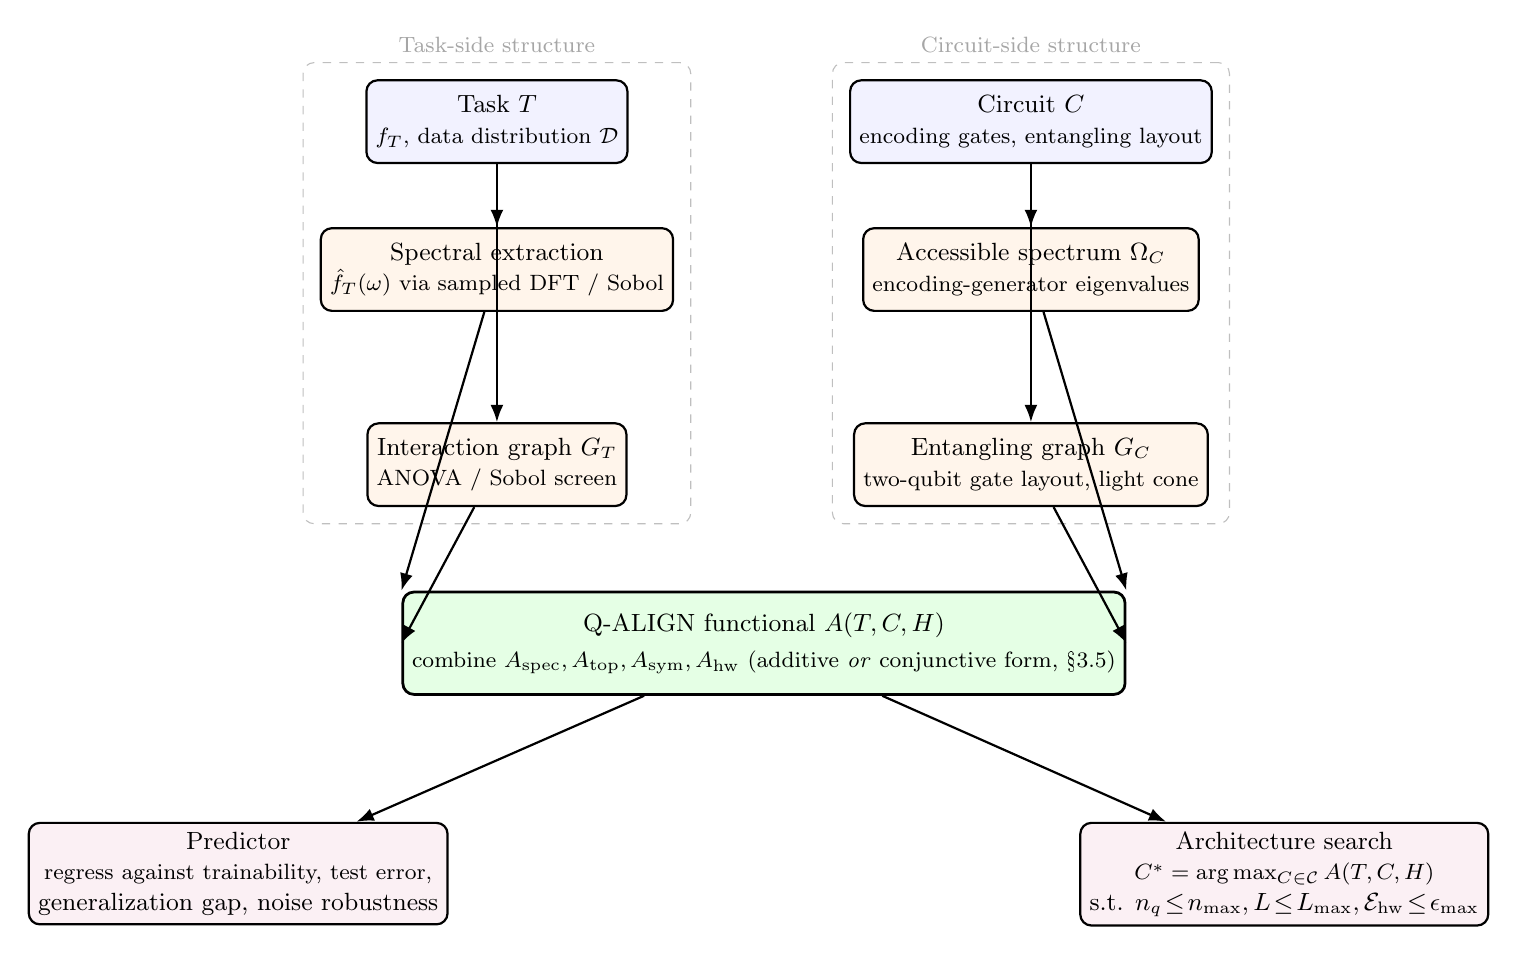
\begin{tikzpicture}[
    node distance=8mm and 12mm,
    font=\small,
    box/.style={draw, rounded corners, align=center, minimum height=1.05cm, minimum width=3.1cm, fill=blue!5, thick},
    proc/.style={draw, rounded corners, align=center, minimum height=1.05cm, minimum width=3.1cm, fill=orange!8, thick},
    score/.style={draw, rounded corners, align=center, minimum height=1.3cm, minimum width=3.6cm, fill=green!10, thick, line width=1pt},
    outbox/.style={draw, rounded corners, align=center, minimum height=1.0cm, minimum width=3.3cm, fill=purple!6, thick},
    arrow/.style={-{Latex[length=2.2mm]}, thick},
    every node/.style={font=\small}
]

% Row 1: Task and Circuit inputs
\node[box] (task) {Task $T$\\ \footnotesize $f_T$, data distribution $\mathcal{D}$};
\node[box, right=28mm of task] (circuit) {Circuit $C$\\ \footnotesize encoding gates, entangling layout};

% Row 2: structural extraction
\node[proc, below=of task] (specextr) {Spectral extraction\\ \footnotesize $\hat f_T(\omega)$ via sampled DFT / Sobol};
\node[proc, below=of circuit] (circspec) {Accessible spectrum $\Omega_C$\\ \footnotesize encoding-generator eigenvalues};

\node[proc, below=14mm of specextr] (topextr) {Interaction graph $G_T$\\ \footnotesize ANOVA / Sobol screen};
\node[proc, below=14mm of circspec] (circtop) {Entangling graph $G_C$\\ \footnotesize two-qubit gate layout, light cone};

% Row 3: alignment terms
\node[score, below=16mm of $(topextr)!0.5!(circtop)$] (align) {Q-ALIGN functional $A(T,C,H)$\\[2pt]
\footnotesize combine $A_{\mathrm{spec}}, A_{\mathrm{top}}, A_{\mathrm{sym}}, A_{\mathrm{hw}}$ (additive \emph{or} conjunctive form, \S3.5)};

% Row 4: outputs
\node[outbox, below left=16mm and -6mm of align] (predict) {Predictor\\ \footnotesize regress against trainability, test error,\\ generalization gap, noise robustness};
\node[outbox, below right=16mm and -6mm of align] (search) {Architecture search\\ \footnotesize $C^\ast = \arg\max_{C\in\mathcal{C}} A(T,C,H)$\\ s.t. $n_q\!\le\! n_{\max}, L\!\le\! L_{\max}, \mathcal{E}_{\mathrm{hw}}\!\le\!\epsilon_{\max}$};

% arrows
\draw[arrow] (task) -- (specextr);
\draw[arrow] (task) -- (topextr);
\draw[arrow] (circuit) -- (circspec);
\draw[arrow] (circuit) -- (circtop);
\draw[arrow] (specextr) -- (align.north west);
\draw[arrow] (circspec) -- (align.north east);
\draw[arrow] (topextr) -- (align.west);
\draw[arrow] (circtop) -- (align.east);
\draw[arrow] (align) -- (predict);
\draw[arrow] (align) -- (search);

% background grouping
\begin{scope}[on background layer]
\node[draw=gray!50, dashed, rounded corners, fit=(task)(specextr)(topextr), inner sep=6pt, label={[gray!70]above:{\footnotesize Task-side structure}}] {};
\node[draw=gray!50, dashed, rounded corners, fit=(circuit)(circspec)(circtop), inner sep=6pt, label={[gray!70]above:{\footnotesize Circuit-side structure}}] {};
\end{scope}

\end{tikzpicture}
\caption{The Q-ALIGN methodology. Task structure (spectral content, variable-interaction graph) and circuit structure (accessible frequency spectrum, entangling graph) are extracted independently and combined --- \emph{before any training} --- into the alignment functional $A(T,C,H)$. The functional is then used either as a pre-training \textbf{predictor} of post-training outcomes (\cref{sec:experiments}, Contribution~2--3) or as a training-free \textbf{objective for architecture search} (\cref{sec:experiments}, Contribution~4).}
\label{fig:pipeline}
\end{figure}

% =======================================================================
\section{Experimental Design}
\label{sec:experiments}
% =======================================================================

\subsection{Task and circuit families}
We will construct at least three structurally distinct task families to avoid single-dataset artifacts:
\begin{enumerate}[leftmargin=1.6em]
    \item \textbf{Periodic/Fourier-heavy regression}, with target functions of controlled, known Fourier support (synthetic) and real-valued signal-regression benchmarks, allowing $\Aspec$ to be computed near-exactly.
    \item \textbf{Graph-structured classification}, with datasets whose class boundary is known (synthetic) or estimated (real) to depend on specific pairwise or higher-order variable interactions, allowing $\Atop$ to be computed against a known or estimated interaction graph.
    \item \textbf{A reinforcement-learning control task}, used for the cross-paradigm stage of the transfer experiment (\cref{sec:transfer}), with a PQC used as a policy or value-function approximator.
\end{enumerate}
For each task family, we will construct circuit families that hold $n_q$, $P$, $L$, $G$ approximately fixed while varying (a) the data-encoding generator set (to vary $\Omc$) and (b) the entangling gate layout (to vary $G_C$), so that $\Aspec$ and $\Atop$ can be driven apart from conventional complexity while conventional complexity is held fixed.

\subsection{Central experiment: complexity-matched separation}
\label{sec:central-experiment}

\paragraph{Avoiding circularity in circuit selection.} A design that hand-picks four circuits \emph{because} they already satisfy $A(C_1)>A(C_2)>A(C_3)>A(C_4)$, drawn from an unconstrained and unreported space of candidates, risks the criticism that the four were selected (consciously or not) to produce the desired separation. We commit to the following protocol, fixed before any training is run, to close this gap:
\begin{enumerate}[leftmargin=1.8em]
    \item \textbf{Independent sampling.} For each task family, we generate a large pool of circuits by independently randomizing the data-encoding generator set and the entangling gate layout within the fixed budget $(n_q, P, L)$, \emph{without reference to their eventual $A$ score at generation time} (i.e., the randomization procedure does not condition on $A$). The pool size $N$ is set by the power analysis below, not fixed arbitrarily.
    \item \textbf{Post-hoc stratification, not selection.} We compute $A$ for every circuit in the pool \emph{after} generation and stratify the pool into quartiles of $A$; the four (or more) circuits reported in \cref{tab:central} are then drawn at random \emph{within} each quartile, rather than hand-picked as the most favorable exemplar of that quartile. \textbf{Which aggregation form defines the quartiles.} Because $A_+$, $A_\times$, and $A_{\min}$ can rank the same pool differently precisely when $\Aspec,\Atop$ are imbalanced (the regime \cref{rem:aggregation-inconsistency} is most concerned with), a quartile boundary is not a form-independent notion, and we must fix one form for defining the stratification itself. We use $A_{\min}(T,C,H)$ for this purpose, for two reasons: (i) it is the most conservative of the three forms, so a circuit placed in the top quartile by $A_{\min}$ is, if anything, an easier case for a search procedure maximizing $A_+$ or $A_\times$ to also have ranked highly, keeping the stratification a conservative rather than favorable choice; and (ii) its core term $\min(\Aspec,\Atop)$ requires no $\alpha,\beta$ weighting at all (only the secondary $\gamma,\delta$ extension weights), so pool stratification does not itself depend on the calibration-fold weight fit of \cref{rem:no-leakage}, avoiding a circular dependency between ``which circuits are sampled for the central experiment'' and ``which fold the weights defining alignment were fit on.'' $A_+$ and $A_\times$ (using the calibration-fold weights of \cref{rem:no-leakage}) are then computed \emph{after} the fact on the same, already-selected circuits, and reported as a supplementary re-ranking within \cref{sec:results}, rather than used to re-select which circuits appear in \cref{tab:central}.
    \item \textbf{Pre-registration.} The randomization procedure, the pool size $N$, the stratification rule (including the choice of $A_{\min}$ as the stratifying form), and the within-quartile sampling seed are fixed and time-stamped before any circuit in the pool is trained, and are reported in full (including circuits that were sampled but not highlighted in the main text) in supplementary material.
    \item \textbf{Whole-pool regression as the primary evidence.} The ordinal comparison of \cref{tab:central} is reported as an illustrative, human-readable instance of the effect, but the \emph{primary} statistical evidence for \cref{sec:central-experiment} is the regression of realized performance against $A$ over the \emph{entire} pool of $N$ circuits (\cref{sec:results}), which is far less susceptible to cherry-picking than a four-point comparison.
\end{enumerate}

\paragraph{Power analysis: sizing the pool for the conditional (covariate-adjusted) regression, not just the marginal one.} A pool of $N=50$, once split across four alignment quartiles and further stratified into (binned) expressibility and entangling-capability cells for the covariate-adjusted analysis of the next paragraph, can leave individual cells with very few circuits --- too few for the covariate-\emph{conditional} test to have adequate power, even if the marginal (unconditional) association between $A$ and performance is real and would have been detected at a smaller $N$. Reporting a non-rejection of $H_0$ from an underpowered conditional analysis would be indistinguishable, to a reader, from a genuine null result, which is precisely the ambiguity a pre-registered protocol is meant to remove. We therefore commit to a pre-registered power analysis, run before $N$ is fixed: we specify a minimum detectable effect size for the conditional regression coefficient on $A$ (e.g., a partial $R^2$ or standardized effect judged to be the smallest effect size of practical interest for an architecture-selection criterion), compute the pool size required for $80\%$ power to detect it at the corrected significance threshold of \cref{rem:multiple-comparisons} given the planned number of covariate strata, and set $N$ to the larger of this requirement and a floor of $N \geq 150$ per task family (raised from the $N\geq 50$ figure used for illustration earlier in this proposal, which we now treat as insufficient once the covariate-stratified analysis is taken into account). Where the resulting $N$ is computationally infeasible within the training-cost budget of \cref{sec:cost}, we will reduce the number of covariate strata (e.g., a single binary split on each covariate rather than quartiles) rather than silently under-power the test, and will state this trade-off explicitly rather than leaving $N$ fixed at a number chosen for convenience.

\paragraph{Controlling for expressibility and entangling capability.} Varying the encoding generator set to change $\Omc$, or varying the entangling layout to change $G_C$, can incidentally change a circuit's expressibility \citep{sim2019expressibility} or effective dimension \citep{abbas2021power} even when $n_q, P, L$ are held fixed --- and either could independently explain a performance difference that we would otherwise (incorrectly) attribute to $A$. We therefore treat expressibility and entangling capability as \emph{controlled covariates}, not merely as post hoc baselines: within each quartile of the sampling procedure above, we additionally stratify on (binned) expressibility and entangling capability, and report the central-experiment regression both unconditionally and conditional on these covariates. If the incremental predictive value of $A$ collapses once expressibility/entangling capability are conditioned on, this must be reported as a genuine negative finding rather than omitted.

The success criterion, evaluated primarily via the whole-pool regression and secondarily via the illustrative ordinal comparison, is that trained performance increases with $A$ despite matched $(n_q,P,L)$ and after conditioning on expressibility and entangling capability:
\[
    A_{\min}(C_1) > A_{\min}(C_2) > A_{\min}(C_3) > A_{\min}(C_4) \;\Longrightarrow\; P(C_1) > P(C_2) > P(C_3) > P(C_4)
\]
for the illustrative quartile-representative circuits of \cref{tab:central} (quartiles defined by $A_{\min}$, per the stratification choice above). The whole-pool regression of \cref{sec:results} is, in contrast, reported for all three aggregation forms, so the primary evidence is not restricted to $A_{\min}$ even though the illustrative table is. This isolates \emph{structure} from \emph{size} (and, via the covariate analysis, from circuit-intrinsic richness) as the explanatory variable, and the entire protocol is repeated independently across the three task families of \cref{sec:experiments} to test whether the pattern is a general property of alignment or an artifact of a single dataset.

\begin{table}[htbp]
\centering
\caption{Template for the complexity-matched central experiment (\cref{sec:central-experiment}): one representative circuit drawn at random from each quartile of the pre-registered, independently sampled pool ($N \geq 150$ per task family, or as set by the pre-registered power analysis if larger; see text). Quartiles (Q1--Q4) are defined by $A_{\min}$ (see text); the ``Alignment'' column reports $A_{\min}$, with $A_+$ and $A_\times$ (computed on the same circuits using calibration-fold weights) reported as a supplementary re-ranking in \cref{sec:results} rather than shown here. $A_{\min}$ values shown are illustrative placeholders consistent with the quartile design; expressibility/entangling-capability bins and $P$ (performance, sign-corrected per \cref{rem:log-hygiene}) are left unfilled until data collection (\cref{sec:results}).}
\label{tab:central}
\begin{tabular}{@{}lccccccc@{}}
\toprule
Architecture & Qubits $n_q$ & Parameters $P$ & Depth $L$ & Alignment $A_{\min}$ & Expr.\ bin & Entangl.\ bin & Performance $P(C)$ \\
\midrule
$C_1$ (Q4) & 8 & 32 & 12 & 0.91 & --- & --- & --- \\
$C_2$ (Q3) & 8 & 32 & 12 & 0.63 & --- & --- & --- \\
$C_3$ (Q2) & 8 & 32 & 12 & 0.41 & --- & --- & --- \\
$C_4$ (Q1) & 8 & 32 & 12 & 0.27 & --- & --- & --- \\
\bottomrule
\end{tabular}
\end{table}

\subsection{Cross-task transfer protocol}
\label{sec:transfer}
We calibrate any fitted components of $A$ (i.e., the weights $\alpha,\beta,\gamma,\delta$ of \cref{def:qalign}, if not fixed from theory) on task family $1,\dots,K-1$ and evaluate predictive strength on a held-out task family $K$ \emph{without recalibration}, at three escalating stages of domain distance:
\begin{enumerate}[leftmargin=1.6em]
    \item within-domain transfer (classification $\rightarrow$ classification, new dataset);
    \item cross-paradigm transfer (classification $\rightarrow$ reinforcement learning);
    \item held-out task-family transfer (an entirely unseen task class, e.g., regression on physical-simulation data or a combinatorial-optimization task).
\end{enumerate}
Predictive strength at each stage is reported via $R^2$ and Kendall's $\tau$, so that degradation of transfer with domain distance is a graded, quantitative claim rather than a binary success/failure.

\paragraph{Pre-registration parity with \cref{sec:central-experiment}.} The central experiment above is held to an explicit pre-registration standard (independent sampling, fixed pool size set by a power analysis, time-stamped protocol); the transfer protocol must be held to the same standard, or its conclusions are not on equal evidentiary footing. We therefore additionally commit, before running any transfer-stage evaluation, to: (i) a pre-registered sample size per stage (number of within-domain datasets, number of cross-paradigm task instances, and number of held-out task-family instances), set by the same power-analysis logic as \cref{sec:central-experiment} rather than by convenience; and (ii) an unbiased, documented selection procedure for the held-out task family of stage 3, since choosing it \emph{because} it is known to work well (or, defensively, because it is known to be hard) would bias the transfer claim in either direction. Concretely, we will fix the candidate set of eligible held-out task families (e.g., a short list of established benchmark task classes external to the three families used for calibration) before designing any part of the Q-ALIGN estimators, and select the actual held-out family from this list by an independent random draw, with the full candidate list and draw procedure reported in supplementary material alongside the central-experiment protocol.

\subsection{Architecture design experiment}
We compare Q-ALIGN-guided search, $C^\ast = \arg\max_{C\in\mathcal{C}} A(T,C,H)$ subject to $n_q \le n_{\max}$, $L \le L_{\max}$, $\mathcal{E}_{\mathrm{hw}} \le \epsilon_{\max}$, against: (i) random architecture sampling; (ii) conventional QAS baselines \citep{du2022quantum,zhang2022differentiable,ostaszewski2021reinforcement}; (iii) depth-based selection; (iv) parameter-count-based selection; and (v), where computationally feasible, exhaustive/brute-force training as an upper-bound reference. The primary metric is \emph{performance achieved per training evaluation}, i.e., the sample efficiency of the search procedure itself, since this is the quantity that would justify replacing (or pre-filtering) a trained-feedback search loop with a training-free structural score. Consistent with the parity commitment of \cref{sec:transfer}, we pre-register, before any method is run: (i) the total training-evaluation budget allotted to each method (the $x$-axis extent of the performance-per-evaluation curves of \cref{sec:results}), fixed and matched across methods rather than chosen after seeing which budget favors Q-ALIGN-guided search; and (ii) the number of independent random seeds per method (search re-runs from different initializations), set by the same power-analysis logic as \cref{sec:central-experiment} so that a comparison showing no significant difference between methods can be attributed to a genuine null result rather than to an under-powered number of seeds.

\subsection{Noise-robustness protocol}
For each circuit evaluated under \cref{sec:central-experiment}, we additionally evaluate performance under a depolarizing-noise sweep (simulated), and, where hardware access permits, a small real-device validation, to test whether $\Ahw(C,H)$ contributes incremental predictive value for noise robustness beyond $\Aspec,\Atop$ alone, and to bound the gap between simulated and real noise conditions. Held to the same pre-registration parity as \cref{sec:transfer,sec:central-experiment}, we fix in advance --- rather than choosing after seeing initial results --- the number and spacing of noise-level points in the sweep (e.g., a pre-specified grid of per-gate depolarizing rates), the number of random seeds per noise level, and, given the substantial expansion of the training-evaluation budget this protocol implies (see \cref{sec:cost}), a pre-registered decision rule for whether the full sweep is run on every circuit in the central-experiment pool or on a stratified sub-sample of it.

\subsection{Computational cost of alignment estimation}
\label{sec:cost}
The claim that Q-ALIGN offers a cheaper alternative to trial training (\cref{sec:results}, architecture-design metric) is only informative if the cost of computing $A(T,C,H)$ itself is measured and shown to be small relative to the training cost it is meant to replace or pre-filter. This is not guaranteed a priori: the sampled-spectral-coverage estimator of $\Aspec$ requires evaluating $\fT$ (or a proxy for it) at enough points to resolve its dominant frequencies, and the Sobol/ANOVA-based estimator of $\Atop$ is well known to suffer from the curse of dimensionality when estimating interaction indices of order two or higher, potentially requiring a sample complexity that is itself substantial for high-dimensional tasks. We therefore commit to reporting, for every task family and circuit family in \cref{sec:experiments}:
\begin{itemize}[leftmargin=1.8em]
    \item the wall-clock and query cost of estimating $\hat\Aspec$ and $\hat\Atop$ (number of function evaluations of $\fT$, or of $\mathcal{D}$-samples, required to reach the bias/variance targets validated in \cref{sec:estimation});
    \item the wall-clock and query cost of a single partial training run of one candidate circuit (i.e., the unit of cost that a trained-feedback search loop such as QAS would spend per candidate);
    \item the resulting ratio, reported per task family, since this ratio --- not the existence of a training-free score in the abstract --- is what would justify the sample-efficiency claim of \cref{sec:experiments} (architecture design experiment). If this ratio is unfavorable for a given task family (i.e., alignment estimation is not substantially cheaper than partial training), we report this as a boundary condition on where Q-ALIGN's efficiency claim holds, consistent with \cref{sec:results}.
\end{itemize}

\paragraph{Total experimental budget: a feasibility check on \cref{sec:central-experiment} as a whole.} The per-comparison cost ratio above is necessary but not sufficient: the power-analysis floor of $N \geq 150$ circuits per task family (\cref{sec:central-experiment}), multiplied across three task families, commits the central experiment alone to partial training of at least $\sim 450$ circuits before the noise-robustness sweep of the preceding subsection is even applied, and that sweep multiplies the per-circuit cost further by the number of noise levels and seeds pre-registered above. We treat this aggregate --- not merely the per-circuit ratio --- as a first-class feasibility question to be resolved \emph{before}, not after, committing to the full campaign: we will estimate the total wall-clock/compute budget implied by ($N\!\ge\!150$ circuits) $\times$ (3 task families) $\times$ (partial-training cost) $\times$ (noise-sweep multiplier), compare it against the compute resources realistically available (i.e., typical academic simulation clusters rather than industrial-scale compute), and, if the budget is infeasible at full scale, apply a pre-registered, explicitly reported fallback \emph{in a fixed priority order} rather than an ad hoc reduction chosen after seeing which cut is most convenient: first reduce the noise-sweep sub-sample fraction (per the decision rule of the preceding subsection), then reduce the number of covariate strata (per \cref{sec:central-experiment}), and only as a last resort reduce $N$ below the power-analysis floor, in which case the resulting loss of power must be reported alongside any resulting non-significant finding rather than left implicit. This ordering is chosen because it degrades the covariate-adjustment and noise-robustness claims before it degrades the core, pre-registered power guarantee of the central experiment itself. The pilot experiment recommended in \cref{sec:conclusion} is intended, in part, to produce the empirical per-circuit cost figures needed to make this budget estimate concrete rather than speculative.

% =======================================================================
\section{Results}
\label{sec:results}
% =======================================================================

This section fixes, in advance of data collection, the structure in which results will be reported. No numerical outcomes are asserted here; each subsection specifies the hypothesis, the statistical test, and the table/figure template to be populated once experiments are run.

\subsection{Falsifiable hypotheses}
\[
    H_0: A(T,C) \text{ provides no incremental predictive information beyond } (n_q, P, L, G).
\]
\[
    H_1: A(T,C) \text{ provides significant incremental predictive information beyond } (n_q, P, L, G).
\]
$H_0$ will be tested, and reported as rejected or not rejected, separately for each of the four outcomes in \cref{sec:results-outcomes} and for each task family, with pooled results reported alongside per-family results.

\begin{remark}[Multiple-comparisons correction]
\label{rem:multiple-comparisons}
The protocol above entails, at minimum, $4$ outcomes $\times$ $3$ task families $\times$ (at least) $2$ statistics ($\Delta R^2$ significance and Kendall's $\tau$) $\times$ up to $3$ aggregation forms (\cref{sec:combined-functional}) tested against $H_0$, i.e., on the order of $70$ nominally distinct hypothesis tests before accounting for the transfer-stage tests of \cref{sec:transfer}. Reporting each at an uncorrected $\alpha=0.05$ threshold would inflate the family-wise Type-I error rate substantially. We therefore commit to: (i) pre-specifying the full set of tests above before data collection, so that the correction is applied to a fixed, declared family of tests rather than to a family chosen after seeing results; (ii) applying a Benjamini--Hochberg false-discovery-rate correction within each outcome $\times$ task-family block as the primary correction, since this is the standard choice for a moderate number of related, non-independent tests and is less conservative than Bonferroni where tests are positively correlated (as $\Delta R^2$ and Kendall's $\tau$ on the same data are); and (iii) additionally reporting the raw (uncorrected) $p$-values and effect sizes alongside the corrected significance flags in every results table of \cref{sec:results}, so that reviewers can apply an alternative correction if they judge ours too permissive or too conservative.
\end{remark}

\subsection{Outcomes to be predicted}
\label{sec:results-outcomes}
\begin{enumerate}[leftmargin=1.6em]
    \item Trainability (gradient-variance / convergence-rate proxy for barren plateaus);
    \item Test performance (task-appropriate metric: accuracy, MSE, or return);
    \item Generalization gap (train $-$ test performance);
    \item Noise robustness (performance degradation under the noise sweep of \cref{sec:experiments}).
\end{enumerate}

\subsection{Reporting template: incremental variance explained}
For each outcome $y$ and task family $f$, we will report
\[
    \Delta R^2_{f} \;=\; R^2_{\text{Q-ALIGN + complexity}} - R^2_{\text{complexity only}},
\]
with significance assessed via a nested-model $F$-test (or likelihood-ratio test), in the format of \cref{tab:results-template-r2}. Every $R^2$ reported in this subsection is computed on the held-out \emph{evaluation fold} of \cref{rem:no-leakage}, using $A$ values computed with weights fit exclusively on the disjoint \emph{calibration fold}; $\Delta R^2$ is never computed on the same circuits used to fit $(\alpha,\beta,\gamma,\delta)$, precluding the mechanical inflation that would otherwise result from evaluating $A$ on the data it was calibrated to fit. ``Performance'' in every column follows the higher-is-better convention of \cref{rem:log-hygiene} (MSE-based outcomes are reported as $-\log(\mathrm{MSE})$), and results are reported for all three aggregation forms ($A_+$, $A_\times$, $A_{\min}$), not only the one used to define the central experiment's illustrative quartiles (\cref{sec:central-experiment}).

\begin{table}[htbp]
\centering
\caption{Reporting template for incremental variance explained (\cref{sec:results}). To be populated after data collection; no entries are populated here.}
\label{tab:results-template-r2}
\begin{tabular}{@{}lccccc@{}}
\toprule
Task family & Outcome & $R^2_{\text{complexity}}$ & $R^2_{\text{Q-ALIGN+complexity}}$ & $\Delta R^2$ & $p$-value \\
\midrule
Periodic regression & Test performance & --- & --- & --- & --- \\
Periodic regression & Generalization gap & --- & --- & --- & --- \\
Periodic regression & Trainability & --- & --- & --- & --- \\
Periodic regression & Noise robustness & --- & --- & --- & --- \\
Graph classification & (all four outcomes) & --- & --- & --- & --- \\
RL control & (all four outcomes) & --- & --- & --- & --- \\
\textit{Pooled} & (all four outcomes) & --- & --- & --- & --- \\
\bottomrule
\end{tabular}
\end{table}

\subsection{Reporting template: rank-prediction comparison}
The most reviewer-facing figure will compare Kendall's $\tau$ between each candidate predictor and realized performance:
\[
    \tau_{\mathrm{Kendall}}(A, P) \quad \text{vs.} \quad \tau_{\mathrm{Kendall}}(n_q, P),\; \tau_{\mathrm{Kendall}}(P_{\text{count}}, P),\; \tau_{\mathrm{Kendall}}(L, P),\; \tau_{\mathrm{Kendall}}(\text{expressibility}, P),
\]
reported per task family as a grouped bar chart with bootstrap confidence intervals (\cref{fig:results-template-tau} placeholder), directly answering whether Q-ALIGN provides rank information that simpler measures do not.

\begin{figure}[htbp]
\centering
\fbox{\parbox{0.7\linewidth}{\centering \vspace{2.2cm} \textit{[Placeholder: grouped bar chart of Kendall's $\tau$ for $A$, $n_q$, $P_{\text{count}}$, $L$, and expressibility against realized performance, one group per task family, with bootstrap 95\% confidence intervals. To be generated from experimental data; not populated in this proposal.]} \vspace{2.2cm}}}
\caption{Reporting template for the rank-prediction comparison (\cref{sec:results}).}
\label{fig:results-template-tau}
\end{figure}

\subsection{Reporting template: central experiment separation}
For the complexity-matched central experiment (\cref{sec:central-experiment}), we will report, per task family, whether the ordering $A(C_1)>A(C_2)>A(C_3)>A(C_4)$ implies $P(C_1)>P(C_2)>P(C_3)>P(C_4)$, together with effect sizes and bootstrap confidence intervals across random circuit re-initializations and training seeds (\cref{tab:central} populated with performance values, plus a companion scatter plot of $A$ vs.\ $P$).

\subsection{Reporting template: cross-task transfer}
For each of the three transfer stages of \cref{sec:transfer}, we will report $R^2$ and Kendall's $\tau$ of the alignment-based predictor on the held-out stage, without recalibration, in the format of \cref{tab:transfer-template}, to make degradation with domain distance an explicit, graded quantity.

\begin{table}[htbp]
\centering
\caption{Reporting template for staged cross-task transfer (\cref{sec:transfer}). To be populated after data collection.}
\label{tab:transfer-template}
\begin{tabular}{@{}lcc@{}}
\toprule
Transfer stage & $R^2$ (held-out) & Kendall's $\tau$ (held-out) \\
\midrule
1. Within-domain (classification $\to$ classification) & --- & --- \\
2. Cross-paradigm (classification $\to$ RL) & --- & --- \\
3. Held-out task family (unseen task class) & --- & --- \\
\bottomrule
\end{tabular}
\end{table}

\subsection{Reporting template: architecture design}
For the architecture-design experiment, we will report performance-per-training-evaluation curves (performance on the $y$-axis, cumulative training evaluations on the $x$-axis) for Q-ALIGN-guided search against random sampling, conventional QAS baselines, depth-based selection, parameter-count-based selection, and the exhaustive-training reference where feasible, one panel per task family.

\subsection{Robustness and failure-case reporting}
Consistent with the evidentiary standard we hold ourselves to, we commit to reporting bootstrap confidence intervals across random circuit re-initializations and training seeds for every quantitative claim above, and to reporting any task/circuit combination for which $H_0$ is \emph{not} rejected, together with a discussion of the likely cause (e.g., a task with weak or diffuse spectral structure, for which $\Aspec$ is uninformative by construction). We treat such failure cases as informative boundary conditions rather than as results to be omitted.

% =======================================================================
\section{Discussion}
\label{sec:discussion}
% =======================================================================

\paragraph{Relationship to barren plateaus and expressibility.} Q-ALIGN is explicitly not a replacement for barren-plateau diagnostics \citep{mcclean2018barren,larocca2024review} or expressibility measures \citep{sim2019expressibility}; it targets a different, complementary question (task--circuit compatibility rather than circuit-intrinsic trainability or uniformity). A circuit can be simultaneously well-aligned to a task ($\Aspec, \Atop$ near 1) and untrainable due to barren plateaus, and \cref{thm:spectral-bound} is explicit that it bounds approximation, not optimization, error. We anticipate the strongest empirical account of trainability will combine $\Aspec$ (approximation feasibility) with a gradient-variance diagnostic (optimization feasibility), and we will report both individually and jointly.

\paragraph{Tractability at scale.} The estimators of \cref{sec:estimation} are the central scalability risk: sampled spectral coverage and Sobol-index-based interaction screening both carry finite-sample bias and variance that could, if uncontrolled, produce spurious alignment scores. We will report estimator bias/variance directly (e.g., against tasks with known closed-form spectra) before using the estimators in any of the experiments of \cref{sec:experiments}.

\paragraph{Weight fitting as a threat to the ``structural theory'' claim.} If $\alpha,\beta,\gamma,\delta$ in \cref{def:qalign} must be extensively refit per task family to achieve predictive power, Q-ALIGN risks collapsing into another fitted heuristic rather than a structural theory. We mitigate this by (i) fixing $\alpha,\beta$ from the theory-derived bound of \cref{thm:spectral-bound} where possible, (ii) treating $\gamma,\delta$ purely as ablation extensions, and (iii) making the no-recalibration constraint of \cref{sec:transfer} the paper's central falsifiability test: if transfer without recalibration fails outside near-identical domains, this should be reported as a graded limitation of the theory rather than suppressed.

\paragraph{Hardware realism.} All noise-robustness claims made from simulated depolarizing-noise sweeps alone should be read as a first-order approximation; real device noise (crosstalk, non-Markovian effects, readout error) may swamp the structural effects Q-ALIGN targets, and we will explicitly bound the simulated-to-real gap wherever hardware access permits, rather than asserting that simulated results generalize to hardware without evidence.

\paragraph{Positioning relative to benchmarking concerns in the field.} \citet{bowles2024better} document that quantum-classical performance comparisons are highly sensitive to experimental-design choices (data encoding, hyperparameter tuning parity, dataset selection). Because Q-ALIGN's central claims are about \emph{ranking} circuits against one another on a fixed task (rather than about quantum-versus-classical comparisons), many of these confounds are attenuated, but not eliminated; we will apply matched tuning budgets across all circuits compared within a single experiment.

\paragraph{Aggregation form is an open question, not a settled design choice.} \Cref{rem:aggregation-inconsistency} identifies a genuine tension between the additive functional of \cref{def:qalign} and the necessary-condition structure proved (or conjectured) in \cref{thm:spectral-bound,conj:topological-bound}: since each core term can independently be sufficient to guarantee failure, an additive score can overstate the alignment of a circuit that is strong on one axis and weak on the other. We treat resolving this --- empirically, via the additive/conjunctive ablation of \cref{sec:combined-functional}, rather than by asserting one form is correct on theoretical grounds alone --- as one of the paper's required deliverables, not an optional robustness check. A related, currently unresolved question is the coarseness of the binary topological indicator (\cref{rem:atop-binary-coarse}): if the weighted variant $\Atop^{\mathrm{w}}$ does not outperform $\Atop^{\mathrm{bin}}$ once expressibility/entangling-capability covariates (\cref{sec:central-experiment}) are controlled for, this would suggest that reachability, rather than representational strength, is the operative quantity, which would itself be an informative and reportable finding about the mechanism of topological alignment.

% =======================================================================
\section{Conclusion}
\label{sec:conclusion}
% =======================================================================

We have proposed Q-ALIGN, a structural alignment framework that reframes quantum machine-learning architecture design from \emph{circuit $\rightarrow$ performance prediction}, evaluated post hoc, to \emph{task structure $\rightarrow$ inductive bias $\rightarrow$ alignment $\rightarrow$ architecture selection/design}, evaluated before training. The framework rests on two theoretically grounded components --- a spectral alignment term with a proven lower bound on irreducible approximation error (\cref{thm:spectral-bound}), built directly on the Fourier-series characterization of parameterized quantum circuits \citep{schuld2021effect}, and a topological alignment term with a stated proof strategy (\cref{conj:topological-bound}) --- combined with modular symmetry and hardware-compatibility extensions. We have detailed a falsifiable evaluation protocol, spanning pre-training prediction, staged cross-task transfer without recalibration, and generative architecture search, together with an explicit commitment to reporting failure cases and boundary conditions. Realizing this programme --- beginning with the pilot complexity-matched experiment of \cref{sec:central-experiment} --- constitutes the empirical core of the full paper.

% =======================================================================
\bibliography{references}

\end{document}
